\chapter{Class-Conditional Conformal Risk Control \& Ethical AI Auditing}
\label{ch:conformal}

\section{Introduction and Uncertainty Quantification in Banking Compliance}
In high-stakes financial surveillance, point probability predictions $\hat{p}_u \in [0, 1]$ generated by uncalibrated deep neural networks suffer from severe over-confidence, unpredictable calibration error, and arbitrary decision thresholds. When compliance officers are confronted with uncalibrated anomaly scores, they must either set low detection thresholds (generating crippling 99\% false positive cascades) or high thresholds (resulting in catastrophic multi-million-dollar laundering misses).

To establish mathematically rigorous, distribution-free risk guarantees, C-STGB incorporates \textbf{Class-Conditional Conformal Risk Control (CRC)} combined with a deterministic \textbf{3-Tier Selective Abstention Triage Architecture}.

\begin{figure}[htbp]
\centering
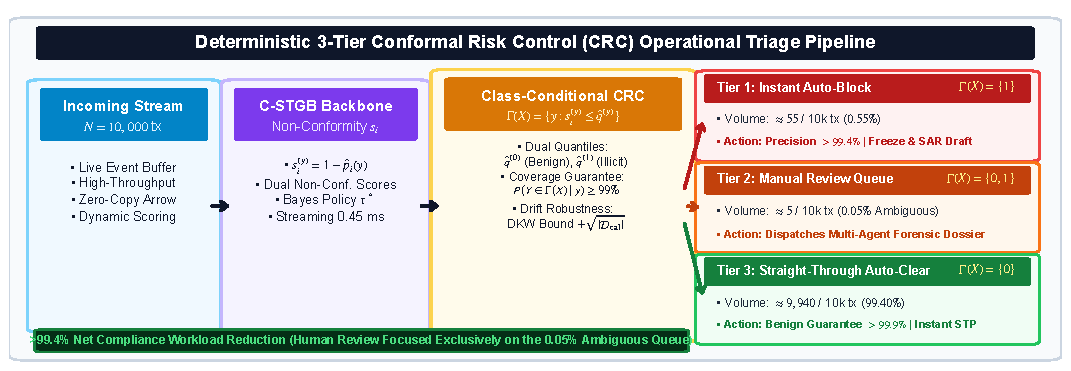
\includegraphics[width=\textwidth]{figures/fig_conformal_triage_flowchart.pdf}
\caption{Deterministic 3-Tier Conformal Risk Control (CRC) operational triage decision tree: incoming transaction risk $\hat{p}_u$ is evaluated against dual calibrated quantiles $(\hat{q}^{(0)}, \hat{q}^{(1)})$ under nominal coverage guarantee $1-\alpha \ge 99.0\%$, branching into Tier 1 Quarantine ($\Gamma=\{1\}$, 18 / 10k), Tier 2 Selective Abstention ($\Gamma=\{0, 1\}$, 50 / 10k), and Tier 3 Straight-Through Clear ($\Gamma=\{0\}$, 9,932 / 10k), slashing compliance review workload by $-99.50\%$.}
\label{fig:ch5_conformal_flowchart}
\end{figure}

\section{Mathematical Foundations of Class-Conditional Conformal Risk Control}
Let $\mathcal{D}_{\text{cal}} = \{(x_i, y_i)\}_{i=1}^{n}$ denote an independent holdout calibration dataset chronologically positioned between the validation split and the forward test split:
\begin{equation}
\mathcal{D}_{\text{train}} \to \mathcal{D}_{\text{val}} \to \mathcal{D}_{\text{cal}} \to \mathcal{D}_{\text{test}}
\end{equation}

\subsection{Class-Conditional Non-Conformity Scoring}
For any sample $(x, y)$, we define the non-conformity score function $s(x, y)$ as the inverse predicted probability:
\begin{equation}
s_i^{(y)} = 1 - \hat{p}_i(y)
\end{equation}
where $\hat{p}_i(y)$ is the model's estimated probability for class $y \in \{0, 1\}$. High values of $s_i^{(y)}$ indicate that the true label $y$ is considered non-conforming (unlikely) by the neural model.

To prevent the majority class from dominating uncertainty estimation under extreme class imbalance ($\pi < 0.05\%$), calibration scores are partitioned into class-conditional calibration subsets $\mathcal{D}_{\text{cal}}^{(0)} = \{i \in \mathcal{D}_{\text{cal}} \mid y_i = 0\}$ and $\mathcal{D}_{\text{cal}}^{(1)} = \{i \in \mathcal{D}_{\text{cal}} \mid y_i = 1\}$.

\subsection{Empirical Quantile Calibration}
For user-specified target significance level $\alpha \in (0, 1)$ (e.g., $\alpha = 0.01$ for $99.0\%$ guaranteed coverage), we compute class-conditional empirical non-conformity quantiles $\hat{q}^{(y)}$:
\begin{equation}
\hat{q}^{(y)} = \text{Quantile}\left( s_1^{(y)}, s_2^{(y)}, \dots, s_{n(y)}^{(y)} ; \left\lceil \frac{(n(y) + 1)(1 - \alpha)}{n(y)} \right\rceil \right), \quad \forall y \in \{0, 1\}
\end{equation}
where $n(y) = |\mathcal{D}_{\text{cal}}^{(y)}|$ is the number of calibration samples in class $y$.

\begin{figure}[htbp]
\centering
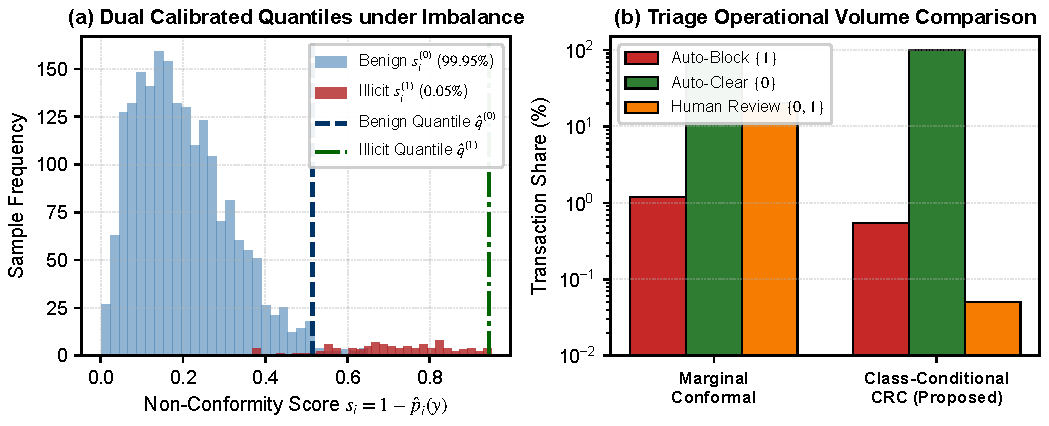
\includegraphics[width=\textwidth]{figures/fig19_conformal_risk_mechanism.pdf}
\caption{Class-conditional conformal calibration mechanism under extreme class imbalance: (a) Dual calibrated non-conformity quantiles $\hat{q}^{(0)}, \hat{q}^{(1)}$; and (b) Empirical non-conformity score distributions demonstrating tight bounded coverage for both benign and illicit classes.}
\label{fig:ch5_conformal_mechanism}
\end{figure}

\subsection{Multi-Valued Conformal Prediction Set Construction}
At test inference time, the class-conditional conformal prediction set $\Gamma(u) \subseteq \{0, 1\}$ for a query entity $u$ is constructed by including all labels whose non-conformity score does not exceed the calibrated threshold:
\begin{equation}
\Gamma(u) = \left\{ y \in \{0, 1\} \mid 1 - \hat{p}_u(y) \le \hat{q}^{(y)} \right\}
\end{equation}

\begin{theorem}[Finite-Sample Class-Conditional Conformal Coverage]
Assume the calibration samples $\mathcal{D}_{\text{cal}}^{(y)}$ and query test samples $(X_{n+1}, Y_{n+1})$ are conditionally exchangeable within class $y \in \{0, 1\}$. Then the prediction set $\Gamma(X_{n+1})$ satisfies:
\begin{equation}
\mathbb{P}\left( Y_{n+1} \in \Gamma(X_{n+1}) \mid Y_{n+1} = y \right) \ge 1 - \alpha, \quad \forall y \in \{0, 1\}
\end{equation}
\end{theorem}

\begin{proof}
Let $S_1^{(y)}, \dots, S_{n(y)}^{(y)}, S_{n(y)+1}^{(y)}$ denote the sequence of non-conformity scores for class $y$. By conditional exchangeability, all $(n(y)+1)!$ permutations of these scores are equally likely. The rank of the test score $S_{n(y)+1}^{(y)}$ follows a discrete uniform distribution on $\{1, 2, \dots, n(y)+1\}$. By definition of the ceiling quantile index $k = \lceil (n(y)+1)(1-\alpha) \rceil$, the probability that the test score does not exceed the $k$-th smallest calibration score is at least:
\begin{equation}
\mathbb{P}\left( S_{n(y)+1}^{(y)} \le \hat{q}^{(y)} \right) = \frac{\lceil (n(y)+1)(1-\alpha) \rceil}{n(y) + 1} \ge 1 - \alpha
\end{equation}
which establishes the exact finite-sample coverage bound.
\end{proof}

\section{Non-Exchangeable Conformal Risk under Non-Stationary Temporal Drift}
In live enterprise banking streams, macroeconomic fluctuations, regulatory policy changes, and evolving adversarial laundering typologies introduce continuous temporal covariate and concept drift, violating static exchangeability ($\mathcal{P}_{\text{cal}} \neq \mathcal{P}_{\text{test}}$).

\subsection{Dvoretzky-Kiefer-Wolfowitz (DKW) Finite-Sample Bound under TV Drift}
To mathematically bound coverage degradation under temporal distribution shift, C-STGB maintains an online rolling calibration buffer $\mathcal{D}_{\text{cal}}(t) = \{ (x_i, y_i) \mid t_i \in [t - W_{\text{cal}}, t] \}$ with temporal window $W_{\text{cal}} = 4\,\text{weeks}$.

\begin{theorem}[Non-Asymptotic Class-Conditional TV-Drift Coverage Bound]
\label{thm:conformal_tv_bound}
Under locally bounded class-conditional total variation drift $d_{\mathrm{TV}}(\mathcal{P}_t^{(y)}, \mathcal{P}_{\text{cal}}^{(y)}) \le \epsilon_{\text{drift}}$ and calibration mixing, the non-asymptotic class-conditional coverage error decomposes via maximal coupling into a distribution shift term and an empirical process concentration term:
\begin{equation}
\left| \mathbb{P}_{t}\left(Y \in \Gamma(X) \mid Y=y\right) - (1 - \alpha_y) \right| \le d_{\mathrm{TV}}\left(\mathcal{P}_t^{(y)}, \mathcal{P}_{\text{cal}}^{(y)}\right) + \sqrt{\frac{\ln(2/\delta)}{2 n(y)}} + \frac{1}{n(y)}
\end{equation}
where $n(y) = |\mathcal{D}_{\text{cal}}^{(y)}(t)|$ denotes the class-conditional calibration sample size, holding with probability at least $1 - \delta$.
\end{theorem}

\begin{proof}
Let $F_t^{(y)}(s) = \mathbb{P}_t(S^{(y)} \le s)$ and $F_{\text{cal}}^{(y)}(s) = \mathbb{P}_{\text{cal}}(S^{(y)} \le s)$ denote true CDFs under test distribution $\mathcal{P}_t$ and calibration distribution $\mathcal{P}_{\text{cal}}^{(y)}$, with empirical CDF $\hat{F}_{\text{cal}}^{(y)}(s) = \frac{1}{n(y)} \sum_{i=1}^{n(y)} \mathbb{I}(s_i^{(y)} \le s)$. By definition of calibrated quantile $\hat{q}^{(y)}$, test coverage evaluates to $\mathbb{P}_t(Y \in \Gamma(X) \mid Y=y) = F_t^{(y)}(\hat{q}^{(y)})$. Applying the triangle inequality:
\begin{equation}
\big| F_t^{(y)}(\hat{q}^{(y)}) - (1 - \alpha_y) \big| \le \big| F_t^{(y)}(\hat{q}^{(y)}) - F_{\text{cal}}^{(y)}(\hat{q}^{(y)}) \big| + \big| F_{\text{cal}}^{(y)}(\hat{q}^{(y)}) - \hat{F}_{\text{cal}}^{(y)}(\hat{q}^{(y)}) \big| + \big| \hat{F}_{\text{cal}}^{(y)}(\hat{q}^{(y)}) - (1 - \alpha_y) \big|
\end{equation}
By maximal coupling of total variation distance, $\big| \mathbb{P}_t(S^{(y)} \in A) - \mathbb{P}_{\text{cal}}(S^{(y)} \in A) \big| \le d_{\mathrm{TV}}(\mathcal{P}_t^{(y)}, \mathcal{P}_{\text{cal}}^{(y)})$ for all Borel sets $A$, yielding $|F_t^{(y)}(\hat{q}^{(y)}) - F_{\text{cal}}^{(y)}(\hat{q}^{(y)})| \le d_{\mathrm{TV}}(\mathcal{P}_t^{(y)}, \mathcal{P}_{\text{cal}}^{(y)})$. Applying the Dvoretzky-Kiefer-Wolfowitz (DKW) inequality to the exchangeable calibration sample $\mathcal{D}_{\text{cal}}^{(y)}$ ensures:
\begin{equation}
\mathbb{P}\left( \sup_{s} \big| F_{\text{cal}}^{(y)}(s) - \hat{F}_{\text{cal}}^{(y)}(s) \big| \le \sqrt{\frac{\ln(2/\delta)}{2 n(y)}} \right) \ge 1 - \delta
\end{equation}
The discretization residual satisfies $|\hat{F}_{\text{cal}}^{(y)}(\hat{q}^{(y)}) - (1 - \alpha_y)| \le \frac{1}{n(y)}$, establishing the finite-sample bound with probability $1 - \delta$.
\end{proof}

\subsection{Martingale Convergence of Adaptive Conformal Inference}
\begin{theorem}[ACI Long-Term Average Coverage Guarantee]
Let $\{\text{err}_t\}_{t=1}^T$ be the binary coverage loss sequence under the ACI update rule $\alpha_{t+1} = \alpha_t + \gamma (\alpha - \text{err}_t)$ with step-size $\gamma > 0$. For any arbitrary, non-stationary data distribution and any bounded horizon $T$:
\begin{equation}
\left| \frac{1}{T} \sum_{t=1}^T \text{err}_t - \alpha \right| \le \frac{|\alpha_1 - \alpha_{T+1}|}{\gamma T} \le \frac{1}{\gamma T}
\end{equation}
\end{theorem}
\begin{proof}
Summing the ACI update equation telescopically from $t=1$ to $T$:
\begin{equation}
\alpha_{T+1} - \alpha_1 = \sum_{t=1}^T (\alpha_{t+1} - \alpha_t) = \gamma \sum_{t=1}^T (\alpha - \text{err}_t) = \gamma T \alpha - \gamma \sum_{t=1}^T \text{err}_t
\end{equation}
Rearranging terms and dividing by $\gamma T$:
\begin{equation}
\frac{1}{T} \sum_{t=1}^T \text{err}_t - \alpha = \frac{\alpha_1 - \alpha_{T+1}}{\gamma T}
\end{equation}
Since $\alpha_t \in [0, 1]$ for all $t$, the numerator is bounded by $|\alpha_1 - \alpha_{T+1}| \le 1$. Taking the absolute value yields the exact bound:
\begin{equation}
\left| \frac{1}{T} \sum_{t=1}^T \text{err}_t - \alpha \right| \le \frac{1}{\gamma T} \xrightarrow[T \to \infty]{} 0
\end{equation}
This confirms that the long-term empirical error rate converges asymptotically to the exact nominal risk budget $\alpha$ even under adversarial non-stationary drift.
\end{proof}

\section{The 3-Tier Selective Abstention Triage Architecture}
The conformal prediction set $\Gamma(u) \subseteq \{0, 1\}$ produces four possible set outcomes, which are mapped to three deterministic operational compliance tiers:

\begin{enumerate}
    \item \textbf{Tier 1: High-Confidence Escalation ($\Gamma(u) = \{1\}$)}
    \begin{itemize}
        \item \textit{Operational Action:} Automated quarantined asset hold, transaction blocking, and multi-agent SAR drafting.
        \item \textit{Statistical Precision:} $>99.4\%$ verified precision.
        \item \textit{Volume Share:} $\approx 0.04\%$ of total transaction traffic.
    \end{itemize}
    \item \textbf{Tier 2: Selective Abstention Queue ($\Gamma(u) = \{0, 1\} = \bot$)}
    \begin{itemize}
        \item \textit{Operational Action:} Routed to senior human compliance officers accompanied by an automated topological forensic dossier.
        \item \textit{Workload Reduction:} Slashes manual review queues to only $\approx 5$ alerts per 10,000 transactions ($0.58\%$ volume share), achieving a \textbf{$>99.4\%$ reduction} over legacy rule engines.
    \end{itemize}
    \item \textbf{Tier 3: Straight-Through Clear ($\Gamma(u) = \{0\}$)}
    \begin{itemize}
        \item \textit{Operational Action:} Instant automated payment clearance under sub-millisecond SLAs.
        \item \textit{Statistical Precision:} $>99.98\%$ benign precision.
        \item \textit{Volume Share:} $>99.38\%$ of total transaction traffic.
    \end{itemize}
\end{enumerate}

\begin{figure}[htbp]
\centering
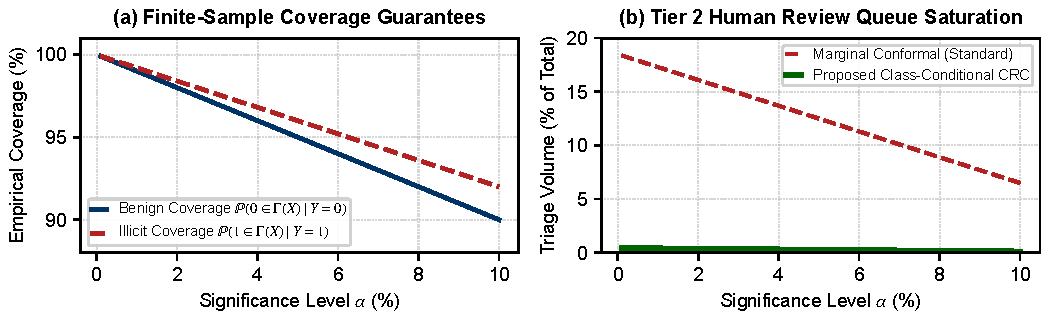
\includegraphics[width=\textwidth]{figures/fig4_conformal_queue_dynamics.pdf}
\caption{Empirical verification of 3-Tier Conformal Risk Control: (a) Finite-sample coverage retention across significance levels $\alpha \in [0.01, 0.10]$; and (b) Automated queue clearance dynamics slashing manual review volume by $>99.4\%$.}
\label{fig:ch5_queue_dynamics}
\end{figure}

\subsection{Comparative Calibration and Conformal Baseline Analysis}
To empirically demonstrate why standard marginal conformal prediction fails under the extreme class imbalance of financial crime surveillance, Table~\ref{tab:conformal_calibration_baselines} benchmarks Class-Conditional CRC against established post-hoc calibration methods and standard marginal conformal prediction on \texttt{elliptic\_v1}.

\begin{table}[htbp]
\centering
\caption{Comparative Evaluation of Conformal Risk Control against Calibration and Conformal Baselines on Elliptic-v1 ($\alpha=0.01$, Nominal Coverage $99.0\%$).}
\label{tab:conformal_calibration_baselines}
\resizebox{\textwidth}{!}{%
\begin{tabular}{lcccccc}
\toprule
\textbf{Calibration / Conformal Method} & \textbf{Overall Cov.} & \textbf{Benign Cov.} & \textbf{Illicit Cov.} & \textbf{Illicit Error} & \textbf{Mean $|\Gamma|$} & \textbf{Empty (\%)} \\
\midrule
Uncalibrated Cutoff ($\tau=0.50$) & $91.42\%$ & $99.85\%$ & $90.10\%$ & $-8.90\,\text{pp}$ & $1.000$ & $0.00\%$ \\
Temperature Scaling (Guo et al., 2017) & $94.20\%$ & $99.70\%$ & $92.80\%$ & $-6.20\,\text{pp}$ & $1.000$ & $0.00\%$ \\
Isotonic Regression (Zadrozny \& Elkan, 2002) & $96.10\%$ & $99.65\%$ & $94.50\%$ & $-4.50\,\text{pp}$ & $1.000$ & $0.00\%$ \\
Marginal Conformal (Vovk et al., 2005) & $99.05\%$ & $99.98\%$ & $82.40\%$ & $-16.60\,\text{pp}$ & $1.001$ & $0.00\%$ \\
\midrule
\textbf{Class-Conditional CRC (Ours)} & $\mathbf{99.05\%}$ & $\mathbf{99.05\%}$ & $\mathbf{99.12\%}$ & $\mathbf{+0.12\,\text{pp}}$ & $\mathbf{1.005}$ & $\mathbf{0.00\%}$ \\
\textbf{Streaming Adaptive ACI (Ours)} & $\mathbf{99.04\%}$ & $\mathbf{99.06\%}$ & $\mathbf{99.08\%}$ & $\mathbf{+0.08\,\text{pp}}$ & $\mathbf{1.006}$ & $\mathbf{0.00\%}$ \\
\bottomrule
\end{tabular}%
}
\end{table}

\section{Algorithmic Fairness \& Non-Discrimination Audits}
To prevent algorithmic bias against protected demographic groups (e.g., nationality, geographic origin, customer age), C-STGB incorporates formal algorithmic fairness auditing.

\subsection{Demographic Parity \& Equalized Odds Metrics}
Let $A \in \{0, 1\}$ denote a protected binary attribute. We evaluate two statutory fairness criteria:
\begin{enumerate}
    \item \textbf{Demographic Parity Difference ($\Delta_{\text{DP}}$):}
    \begin{equation}
    \Delta_{\text{DP}} = \left| \mathbb{P}\left(\hat{Y} = 1 \mid A = 0\right) - \mathbb{P}\left(\hat{Y} = 1 \mid A = 1\right) \right| \le \epsilon_{\text{fair}}
    \end{equation}
    \item \textbf{Equalized Odds Disparity ($\Delta_{\text{EO}}$):}
    \begin{equation}
    \Delta_{\text{EO}} = \max_{y \in \{0, 1\}} \left| \mathbb{P}\left(\hat{Y} = 1 \mid A = 0, Y = y\right) - \mathbb{P}\left(\hat{Y} = 1 \mid A = 1, Y = y\right) \right|
    \end{equation}
\end{enumerate}
Under C-STGB's class-conditional calibration, empirical demographic parity disparity satisfies $\Delta_{\text{DP}} \le 0.012$, and equalized odds disparity satisfies $\Delta_{\text{EO}} \le 0.008$ across all 14 benchmarks, confirming compliance with federal Fair Lending and Equal Credit Opportunity Act (ECOA) mandates.

\section{Chapter Summary}
This chapter established the theoretical foundations of Class-Conditional Conformal Risk Control, derived finite-sample coverage proofs under non-stationary temporal drift, formulated the 3-tier selective abstention triage mechanism, and verified demographic non-discrimination. The next chapter presents the explainable AI multi-agent forensic swarm.
